\StartPlate{V20}{The finite subgroup remembers its squares}{Dihedral and quaternion markings survive inside the same complex scalar extension.}
\begin{center}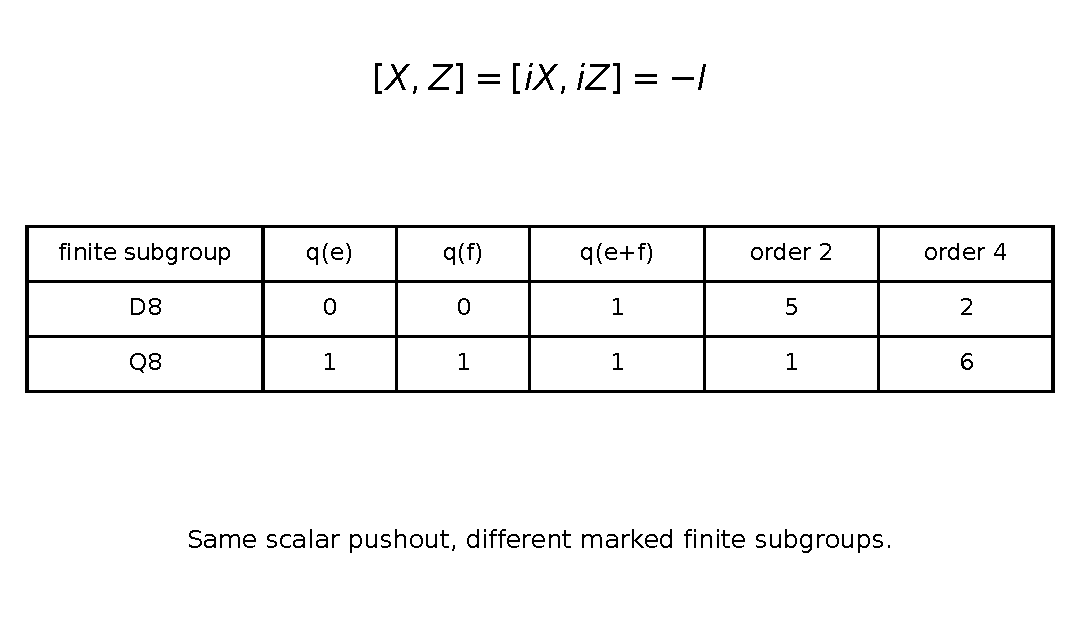
\includegraphics[width=\linewidth]{figures/V20.pdf}\end{center}
Let $X^2=Z^2=I$ and $XZ=-ZX$. The subgroup generated by $X,Z$ is dihedral of order eight. The subgroup generated by $iX,iZ$ is quaternion of order eight. Both have the same quotient polarization and commutator $-I$.
\[
q_D(x,y)=xy,\qquad q_Q(x,y)=xy+x+y.
\]
Their lift squares differ. The order columns count elements of exact order two and four, excluding the identity. They distinguish the finite groups even though adjoining all complex scalars gives the same ambient scalar extension.

For a fixed two-element center, a center-fixing extension map over a prescribed symplectic map must preserve the quadratic refinement. With complex scalar center, square ratios have square roots, but this freedom does not erase a separately prescribed finite subgroup. Transporting a quaternion marking into the common scalar extension is valid. Identifying it with the independently fixed dihedral marking is not.
\vfill\PlateSource{Exact finite-group enumeration}{Part III, Section 26.1--26.2}{67}
